\documentclass[journal,12pt,twocolumn]{IEEEtran}
\usepackage{romannum}
\usepackage{float}
\usepackage{setspace}
\usepackage{gensymb}
\singlespacing
\usepackage[cmex10]{amsmath}
\usepackage{amsthm}
\usepackage{mathrsfs}
\usepackage{txfonts}
\usepackage{stfloats}
\usepackage{bm}
\usepackage{cite}
\usepackage{cases}
\usepackage{subfig}
\usepackage{longtable}
\usepackage{multirow}
\usepackage{enumitem}
\usepackage{mathtools}
\usepackage{steinmetz}
\usepackage{tikz}
\usepackage{circuitikz}
\usepackage{verbatim}
\usepackage{tfrupee}
\usepackage[breaklinks=true]{hyperref}
\usepackage{tkz-euclide}
\usetikzlibrary{calc,math}
\usepackage{listings}
    \usepackage{color}                                            %%
    \usepackage{array}                                            %%
    \usepackage{longtable}                                        %%
    \usepackage{calc}                                             %%
    \usepackage{multirow}                                         %%
    \usepackage{hhline}                                           %%
    \usepackage{ifthen}                                           %%
  %optionally (for landscape tables embedded in another document): %%
    \usepackage{lscape}     
\usepackage{multicol}
\usepackage{chngcntr}
\DeclareMathOperator*{\Res}{Res}
\renewcommand\thesection{\arabic{section}}
\renewcommand\thesubsection{\thesection.\arabic{subsection}}
\renewcommand\thesubsubsection{\thesubsection.\arabic{subsubsection}}

\renewcommand\thesectiondis{\arabic{section}}
\renewcommand\thesubsectiondis{\thesectiondis.\arabic{subsection}}
\renewcommand\thesubsubsectiondis{\thesubsectiondis.\arabic{subsubsection}}

% correct bad hyphenation here
\hyphenation{op-tical net-works semi-conduc-tor}
\def\inputGnumericTable{}                                 %%

\lstset{
frame=single, 
breaklines=true,
columns=fullflexible
}

\begin{document}


\newtheorem{theorem}{Theorem}[section]
\newtheorem{problem}{Problem}
\newtheorem{proposition}{Proposition}[section]
\newtheorem{lemma}{Lemma}[section]
\newtheorem{corollary}[theorem]{Corollary}
\newtheorem{example}{Example}[section]
\newtheorem{definition}[problem]{Definition}
\newcommand{\BEQA}{\begin{eqnarray}}
\newcommand{\EEQA}{\end{eqnarray}}
\newcommand{\define}{\stackrel{\triangle}{=}}

\bibliographystyle{IEEEtran}
\providecommand{\mbf}{\mathbf}
\providecommand{\pr}[1]{\ensuremath{\Pr\left(#1\right)}}
\providecommand{\qfunc}[1]{\ensuremath{Q\left(#1\right)}}
\providecommand{\sbrak}[1]{\ensuremath{{}\left[#1\right]}}
\providecommand{\lsbrak}[1]{\ensuremath{{}\left[#1\right.}}
\providecommand{\rsbrak}[1]{\ensuremath{{}\left.#1\right]}}
\providecommand{\brak}[1]{\ensuremath{\left(#1\right)}}
\providecommand{\lbrak}[1]{\ensuremath{\left(#1\right.}}
\providecommand{\rbrak}[1]{\ensuremath{\left.#1\right)}}
\providecommand{\cbrak}[1]{\ensuremath{\left\{#1\right\}}}
\providecommand{\lcbrak}[1]{\ensuremath{\left\{#1\right.}}
\providecommand{\rcbrak}[1]{\ensuremath{\left.#1\right\}}}
\theoremstyle{remark}
\newtheorem{rem}{Remark}
\newcommand{\sgn}{\mathop{\mathrm{sgn}}}
\providecommand{\abs}[1]{\left\vert#1\right\vert}
\providecommand{\res}[1]{\Res\displaylimits_{#1}} 
\providecommand{\norm}[1]{\left\lVert#1\right\rVert}
\providecommand{\mtx}[1]{\mathbf{#1}}
\providecommand{\mean}[1]{E\left[ #1 \right]}
\providecommand{\fourier}{\overset{\mathcal{F}}{ \rightleftharpoons}}
\providecommand{\system}{\overset{\mathcal{H}}{ \longleftrightarrow}}
\newcommand{\solution}{\noindent \textbf{Solution: }}
\newcommand{\cosec}{\,\text{cosec}\,}
\providecommand{\dec}[2]{\ensuremath{\overset{#1}{\underset{#2}{\gtrless}}}}
\newcommand{\myvec}[1]{\ensuremath{\begin{pmatrix}#1\end{pmatrix}}}
\newcommand{\mydet}[1]{\ensuremath{\begin{vmatrix}#1\end{vmatrix}}}
\numberwithin{equation}{subsection}
\makeatletter
\@addtoreset{figure}{problem}
\makeatother

\let\StandardTheFigure\thefigure
\let\vec\mathbf
\renewcommand{\thefigure}{\theproblem}



\def\putbox#1#2#3{\makebox[0in][l]{\makebox[#1][l]{}\raisebox{\baselineskip}[0in][0in]{\raisebox{#2}[0in][0in]{#3}}}}
     \def\rightbox#1{\makebox[0in][r]{#1}}
     \def\centbox#1{\makebox[0in]{#1}}
     \def\topbox#1{\raisebox{-\baselineskip}[0in][0in]{#1}}
     \def\midbox#1{\raisebox{-0.5\baselineskip}[0in][0in]{#1}}

\vspace{3cm}


\title{Assignment 5}
\author{Jaswanth Chowdary Madala}


% make the title area
\maketitle

\newpage

%\tableofcontents

\bigskip

\renewcommand{\thefigure}{\theenumi}
\renewcommand{\thetable}{\theenumi}

\begin{enumerate}
\item An arch is in the form of a parabola with its axis vertical. The arch is 10 m high and 5 m wide at the base. How wide is it 2 m from the vertex of the parabola?
\begin{figure}[ht]
\centering
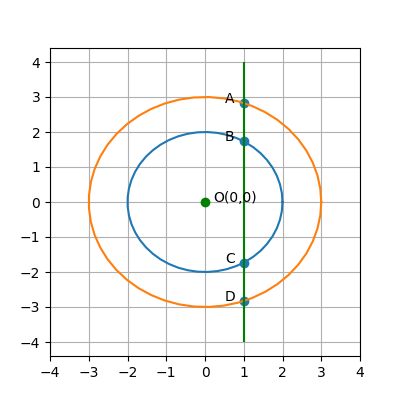
\includegraphics[width = \columnwidth]{"figs/fig.png"}
\caption{Graph}
\label{fig:1}
\end{figure}

\textbf{Solution:} The equation of the conic with focus $\vec{F}$, directrix $\vec{n}^\top\vec{x} = c$ and eccentricity $e$ is given by
\begin{align}
\vec{x}^\top\vec{V}\vec{x} + 2\vec{u}^\top\vec{x} + f = 0
\label{eq:1}
\end{align}
where
\begin{align}
\vec{V} &\triangleq \norm{\vec{n}}^2\vec{I} - e^2\vec{n}\vec{n}^\top \label{eq:2} \\
\vec{u} &\triangleq ce^2\vec{n} - \norm{\vec{n}}^2\vec{F} \label{eq:3} \\
f &\triangleq \norm{\vec{n}}^2\norm{\vec{F}}^2 - c^2e^2 \label{eq:4}
\end{align}
Given that the arch is in the form of parabola, axis is vertical 
\begin{align}
e &= 1 \label{eq:5} \\
\vec{n} &= \myvec{0\\1} \label{eq:6}
\end{align}
Without loss of generality, assume the vertex $\vec{v}$ to be at origin,
\begin{align}
\vec{v} = \myvec{0\\0}
\end{align}
As the point $\vec{v}$ satisfies \eqref{eq:1}, and this gives
\begin{align}
f = 0
\end{align}
Substituting \eqref{eq:5}, \eqref{eq:6} in the equaiton \eqref{eq:2}, it gives
\begin{align}
\vec{V} = \myvec{1&0\\0&0}
\end{align}
Given that arch is 10m high and 5m wide at the base, since the parabola is symmetric to the axis of the parabola, The points
\begin{align}
\vec{P} = \myvec{\frac{5}{2}\\ -10}, \, \vec{Q} = \myvec{-	\frac{5}{2}\\ -10}
\end{align}
satisfies the equation \eqref{eq:1}. \\
Substituting the point $\vec{P}$ in \eqref{eq:1} gives,
\begin{align}
\frac{25}{4} + 2\vec{u}^\top \myvec{\frac{5}{2}\\ -10} &= 0\\
\implies \myvec{4&-16}\vec{u} = -5\label{eq:7}
\end{align}
Substituting the point $\vec{Q}$ in \eqref{eq:1} gives,
\begin{align}
\frac{25}{4} + 2\vec{u}^\top \myvec{-\frac{5}{2}\\ -10} &= 0\\
\implies \myvec{-4&-16}\vec{u} = -5\label{eq:8}
\end{align}
Writing the equations \eqref{eq:7}, \eqref{eq:8} in matrix form gives,
\begin{align}
\myvec{4&-16\\-4&-16}\vec{u} = \myvec{-5\\-5}\label{eq:9}
\end{align}
The augmented matrix for the system equations in \eqref{eq:9} is expressed as
\begin{align}
	\myvec{4&-16&\vrule&-5\\ -4&-16&\vrule&-5} \\
	\xleftrightarrow[]{R_2\leftarrow R_2+R_1}
	\myvec{4&-16&\vrule&-5\\ 0&-32&\vrule&-10} \label{eq:10}
\end{align}
The augmented matrix for the system equations is reduced to Row echelon form, From the above equation \eqref{eq:10} we get the vector $\vec{u}$ as
\begin{align}
\vec{u} = \myvec{0\\\frac{5}{16}}
\end{align}
To find the the how wide the arch at 2m from the vertex of the parabola, we first find the points of intersection $\vec{A}, \vec{B}$ of the line and the parabola 
\begin{align}
\vec{x} = \myvec{0\\-2} + \mu \myvec{1\\0} \label{eq:11}\\
\vec{x}^\top \myvec{1&0\\0&0}\vec{x} + 2\myvec{0\\\frac{5}{16}}^\top \vec{x}= 0\label{eq:12}
\end{align}

The parameter $\mu$ of the points of intersection of line \eqref{eq:13} with the conic section \eqref{eq:14}
\begin{align}
\vec{x} &= \vec{h} + \mu \vec{m}
\label{eq:13}\\
\text{g}\brak{\vec{x}} &= \vec{x}^{\top}\vec{V}\vec{x}+2\vec{u}^{\top}\vec{x}+f=0
\label{eq:14}
\end{align}
is given by the equation 
\begin{align}
\mu^2\vec{m}^{\top}\vec{V}\vec{m} + 2 \mu\vec{m}^{\top}\brak{\vec{V}\vec{h}+\vec{u}} 
	+ \text{g}\brak{\vec{h}} &=0
\label{eq:15}
\end{align}
Here from \eqref{eq:11}, \eqref{eq:12} we get,
\begin{align}
\vec{m}^{\top}\vec{V}\vec{m} & = 1\\
\vec{m}^{\top}\brak{\vec{V}\vec{h}+\vec{u}} &= 0 \\
\text{g}\brak{\vec{h}} &= -\frac{5}{4}
\end{align}
From \eqref{eq:15} we get,
\begin{align}
\mu^2 - \frac{5}{4} &=0\\
\mu &= \pm \frac{\sqrt5}{2}\\
\vec{A} &= \myvec{0\\-2} + \frac{\sqrt5}{2} \myvec{1\\0}\\
&= \myvec{\frac{\sqrt5}{2} \\ -2}\\
\vec{B} &= \myvec{0\\-2} - \frac{\sqrt5}{2} \myvec{1\\0}\\
&= \myvec{-\frac{\sqrt5}{2} \\ -2}
\end{align}
The required width is given by,
\begin{align}
w &= \norm{\vec{A} - \vec{B}}\\
&= \norm{\myvec{\sqrt{5}\\0}}\\
&= \sqrt{5}
\end{align}

\begin{table}[h]
\centering
%%%%%%%%%%%%%%%%%%%%%%%%%%%%%%%%%%%%%%%%%%%%%%%%%%%%%%%%%%%%%%%%%%%%%%
%%                                                                  %%
%%  This is a LaTeX2e table fragment exported from Gnumeric.        %%
%%                                                                  %%
%%%%%%%%%%%%%%%%%%%%%%%%%%%%%%%%%%%%%%%%%%%%%%%%%%%%%%%%%%%%%%%%%%%%%%

\begin{center}
\begin{tabular}{|c|c|c|}
\hline
\textbf{RV}& \textbf{Values} & \textbf{Description} \\ \hline
$X$		   & 	$\{0,1\}$	&  1st draw - 0: black card, 1: red card\\ \hline
$Y$ 		   & 	$\{0,1\}$	&  2nd draw - 0: black card, 1: red card\\ \hline
$X,Y$ 		   & 	$\{00\}$	&	2 cards drawn are black\\ \hline
\end{tabular}
\end{center}

\caption{}
\label{tab:1}
\end{table}

\end{enumerate}
\end{document}
